%!TEX root = report.tex
\chapter{Methodology}
\label{ch:concept_design}
\section{Objectives}
\par We aim to quantify the deviation in bus journey times from the official timetable, so as to improve the prediction of bus travel time downstream from location of last observation in mixed traffic operations. We achieved this by providing 1) a data service \acrshort{api} of bus travel time that provides historical, current, and reference bus timetables, and 2) a demonstrative web application to show case the use of the \acrshort{api}.

\section{Bus Journey Times}
\par The bus journey time for a given route depends on many unpredictable external factors. These include weather conditions, passenger flow, temporary lane closures, as well as the time of the bus trip. Predicting bus journey times by discovering and analysing these contributing factors is complicated.

\par We decided to bypass looking at these factors, and examined the historical and current bus travel times instead. We assumed that for a specific short time frame, the external factors remain largely unchanged. Also, the bus journey times between any two stops on a route is the sum of the travel times between any pair of neighbouring stops. In this case, the bus travel time between a given pair of neighbouring stops is similar to the previous trips performed in the same time frame.

\par For bus journey time between every pair of neighbouring stop at each hour of the day, we provide estimations for the following:
\begin{itemize}
  \item \textbf{Reference Timtable} How long does TfL says it take?
  \item \textbf{Current Timetable} How long does it currently take?
  \item \textbf{Historical Timetable} How long does it usually take?
\end{itemize}

\par Since the reference timetable shows the typical bus journey time, the historical timetable should converge to the reference timetable over time. The current timetable shows the most relevant bus travel time at the observation point, a significant increase in travel time compared to the historical or reference timetables would indicate a bus delay.

\subsection{Reference Timetable}
\par We extracted the average bus travel time between every pair of neighbouring stops for every route during every hour of the day for every day of the week from the \acrshort{tfl} Journey Planner Bus Timetables. This is discussed in Section \ref{sec: official_tfl_timetable}.

\subsection{Current Timetable}
\par We collected the live bus arrival times for the past 1 hour, and stored the final bus arrival times for each bus at each stop. We then found out the travel time of each bus between every pair of neighbouring stops for the given hour. Next, we calculated the average travel time between each pair of neighbouring bus stops. This serves as a prediction for how long the bus currently takes to travel between two neighbouring stops. See implementation details in Section \ref{sec:current_timetable_generation}.

\subsection{Historical Timetable}
\par We stored the current timetable generated at each hour, and grouped them by the hour of the day for the same day of the week. We then calculated the average bus travel time between each pair of neighbouring stops for each hour of the day in each day of the week. For example, the average bus travel time between stop A and stop B for 3pm on Wednesday is the average travel time for all the bus trips between these two stops between 2pm to 3pm in the past Wednesdays. More details can be found in Section \ref{sec:historical_timetable}.

\section{Contributions}
\par We provided the above mentioned three timetables as a data service API (Chapter \ref{ch:data_service}) and designed a demonstrative web application that allows users to check current bus delays from a given bus stop (Chapter \ref{ch:mobile_app}).

\section{Architecture Design}
\par The architecture overview is shown in Figure \ref{fig:architecture}. We discuss each component in detail in the following chapters.

\begin{figure}
\centering
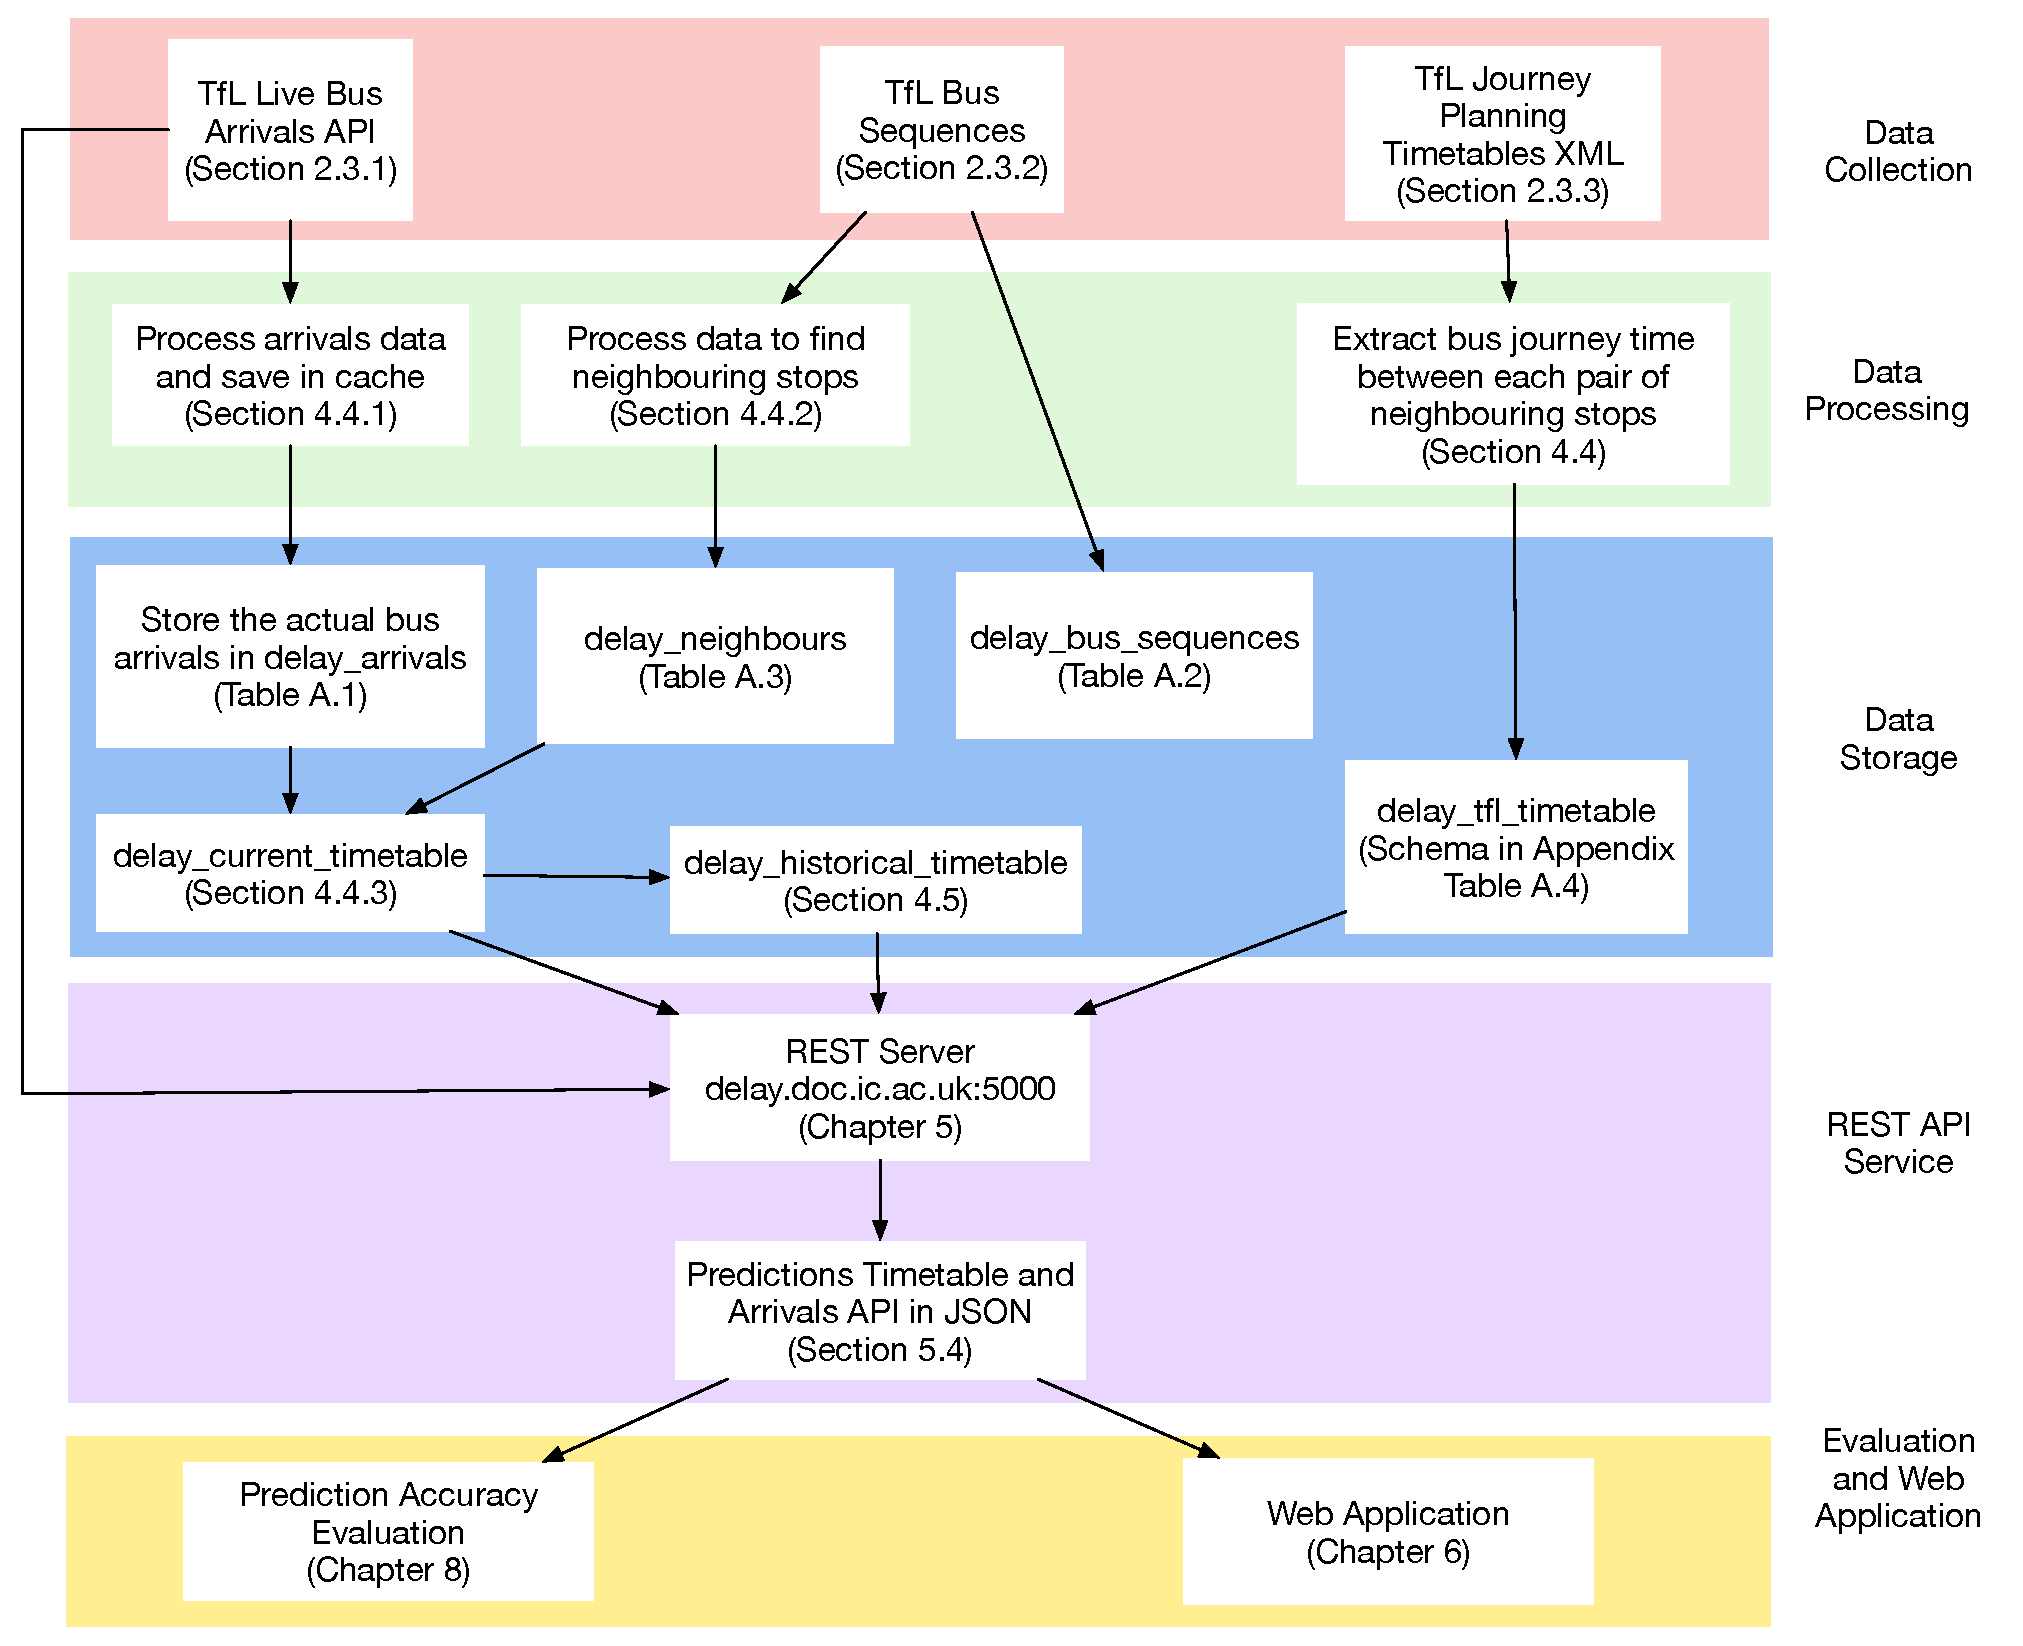
\includegraphics[width=\textwidth]{figures/architecture.pdf}
\caption{\label{fig:architecture} Architecture Overview}
\end{figure}





